\chapter{ADR Dataset Analysis}
    For the analysis of the ADRs, and to answer the research questions, several topic modelling techniques and algorithms were used as mentioned in chapter 4. This section presents the two approaches that led to the final results.
        
    \section{Analysis Using TF-IDF and LDA}
        A first approach employed Term Frequency-Inverse Document Frequency (TF-IDF) for vectorization of words and Latent Dirichlet Allocation (LDA) to perform the topic modelling. TF-IDF is a statistical measure used to evaluate the importance of a word in a document relative to a collection of documents. By applying TF-IDF, each document is converted into a numerical vector, where each element of the vector represents the TF-IDF score of a term, which in extension is essentially the product of TF, the frequency of a a term appearing in a document and IDF, a metric of importance of the term across all documents. After documents have been vectorized, we can apply LDA which is is a generative probabilistic model that assumes documents are mixtures of topics and topics are mixtures of words \cite{LDA_paper}. LDA assumes each document is generated from a fixed number of topics, and each topic is a distribution over a certain fixed vocabulary. The result of this method is a distribution of topics for each ADR, indicating the prevalence of each topic within itself. TF-IDF is used since LDA expects the input in the form of integers and TF-IDF accomplishes just that, along with encoding information about words in the documents. Hyper parameter tuning using grid search was performed to obtain the best parameters, namely max features of TF-IDF, the optimal number of LDA components, and LDA learning decay. This resulted in four broad topics discovered. The topics were projected in a 2 dimensional space and visualized in \ref{fig:LDA_results}. All algorithms were executed using Python and visualized using the pyLDAvis library. When interpreting topics, the top ten words by frequency in each cluster were used.

        \begin{enumerate}
            \item 34.98\% of the documents were represented with the following most common words: ``data'', ``api'', ``user'', ``event'', ``service'', ``type'', ``message'', ``request'', ``object'', ``client''. This topic is broad and could potentially revolve around decisions about how APIs manage, process, and integrate data. This is topic 1 in figure \ref{fig:LDA_results}.
            
            \item 32.62\% of the documents were represented with the following most common words: ``test'', ``component'', ``code'', ``project'', ``library'', ``file'', ``framework'', ``version'', ``package'', ``change''. This topic seems to revolves around decisions on the processes, tools, and practices involved in software testing and development. This is topic 2 in figure \ref{fig:LDA_results}.
    
            \item 25.51\% of the documents were represented with the following most common words: ``aws'', ``service'', ``environment'', ``docker'', ``cluster'', ``container'', ``image'', ``kubernetes'', ``cloud'', ``deployment''. Based on these results this topic is more clear and revolves around decisions about cloud infrastructure containers and container orchestration. This is topic 3 in figure \ref{fig:LDA_results}.
    
            \item 6.89\% of the documents were represented with the following most common words: ``record'', ``database'', ``search'', ``architecture'', ``adrs'', ``architectural'', ``markdown'', ``elasticsearch'', ``index'' ``document'', ``adr'', ``article''. This topic is more intertwined and seems to contain ADRs about the use of ADRs and database decisions. This is topic 4 in figure \ref{fig:LDA_results}.
        \end{enumerate}

        \begin{figure}[ht]
            \centering
            \includegraphics[scale=0.25]{figures/LDA-results/lda_topics_no_info_cleaned.png}
            \caption{Topic Distance Map Identified by TF-ID and LDA using PCA}
            \label{fig:LDA_results}
        \end{figure}

        LDA served as the base for some further exploration and optimization of employed techniques. While the initial topics generated were not entirely clear, they highlighted the necessity for finer categorization into more specific topics that LDA alone could not effectively capture, even after tuning with many parameter combinations. This was evident as attempting to increase the number of topics resulted in significant noise and incoherence. To address this, other models were introduced and applied, presented in the following subsection.

    \section{Analysis Using BERTopic}
        The second approach utlilized the Python library BERTopic \cite{bertTopic} to analyze the contents of the ADRs. BERTopic uses transformer-based language models and a class-based TF-IDF variation to generate coherent topic representations. The whole procedure and the algorithms used for the final analysis can be broken down to the steps below:

        \begin{enumerate}
            \item Document embeddings are generated using pre-trained models to capture semantic similarities, ensuring that documents with similar topics are close in vector space. In order to produce rich embeddings, the ``all-mpnet-base-v2`` transformer model \footnote{https://huggingface.co/sentence-transformers/all-mpnet-base-v2} from Hugging-Face was used for its support of longer documents up to sequences of 512 tokens and due to the fact that it was trained on datasets related to software engineering such as CodeSearchNet\footnote{https://huggingface.co/datasets/code-search-net/code\_search\_net}, that contains over 2 million (comment, code) pairs and StackExchange questions.
            
            \item These embeddings are then reduced in dimensionality to make the clustering process more efficient. For this, the UMAP method was used as it ``keeps some of a dataset's local and global structure``\footnote{https://maartengr.github.io/BERTopic/algorithm/algorithm.html\#2-dimensionality-reduction} which is important to keep as it contains the information necessary to create clusters of semantically similar documents. This technique introduces randomness into the procedure so a set seed was used to make results reproducible.

            \item Clustering is then performed with the reduced embeddings to separate the documents. For this, HDBSCAN was used. This technique was chosen as it can handle varying densities and can also identify outliers, that do not get assigned to a particular topic. Information of this kind is useful for RQ3. The minimum cluster size hyperparameter, which is the main determinant for the number of  topics the model identifies, was set to 40 or about one\% of total ADRs, as smaller numbers produced very distributed niche topics, that related to specific technologies or tools without providing much information about the context or architecture. A larger minimum cluster size on the other hand, produced incoherent clusters without clear separation.

            \item A bag-of-words representation is then created using all documents in the clusters by counting how often each word appears in each collection. This is important since popular words at the cluster level are needed for the analysis. 

            \item Finally, from the generated bag-of-words representation, TF-IDF is applied again, at a cluster level highlighting important words within a cluster and producing a label. Since we now have a set of representative words for each cluster along with the associated documents a fine-tuning technique was used using OpenAI's model GPT-3.5. Specifically, using a custom prompt, the main set of words for each cluster along with the four documents closest to the center of the cluster were passed as input to the LLM, prompting it to generate characteristic labels for this cluster using natural language. The prompt also contained context of the analysis, stating that the document collection consisted of ADRs, which are part of software engineering.
            
        \end{enumerate}
        
        
    \section{Analysis Results}
        The first form of the analysis' results are presented in figure \ref{fig:bertopic_datamap_original}.

        \begin{figure}[h]
            \centering
            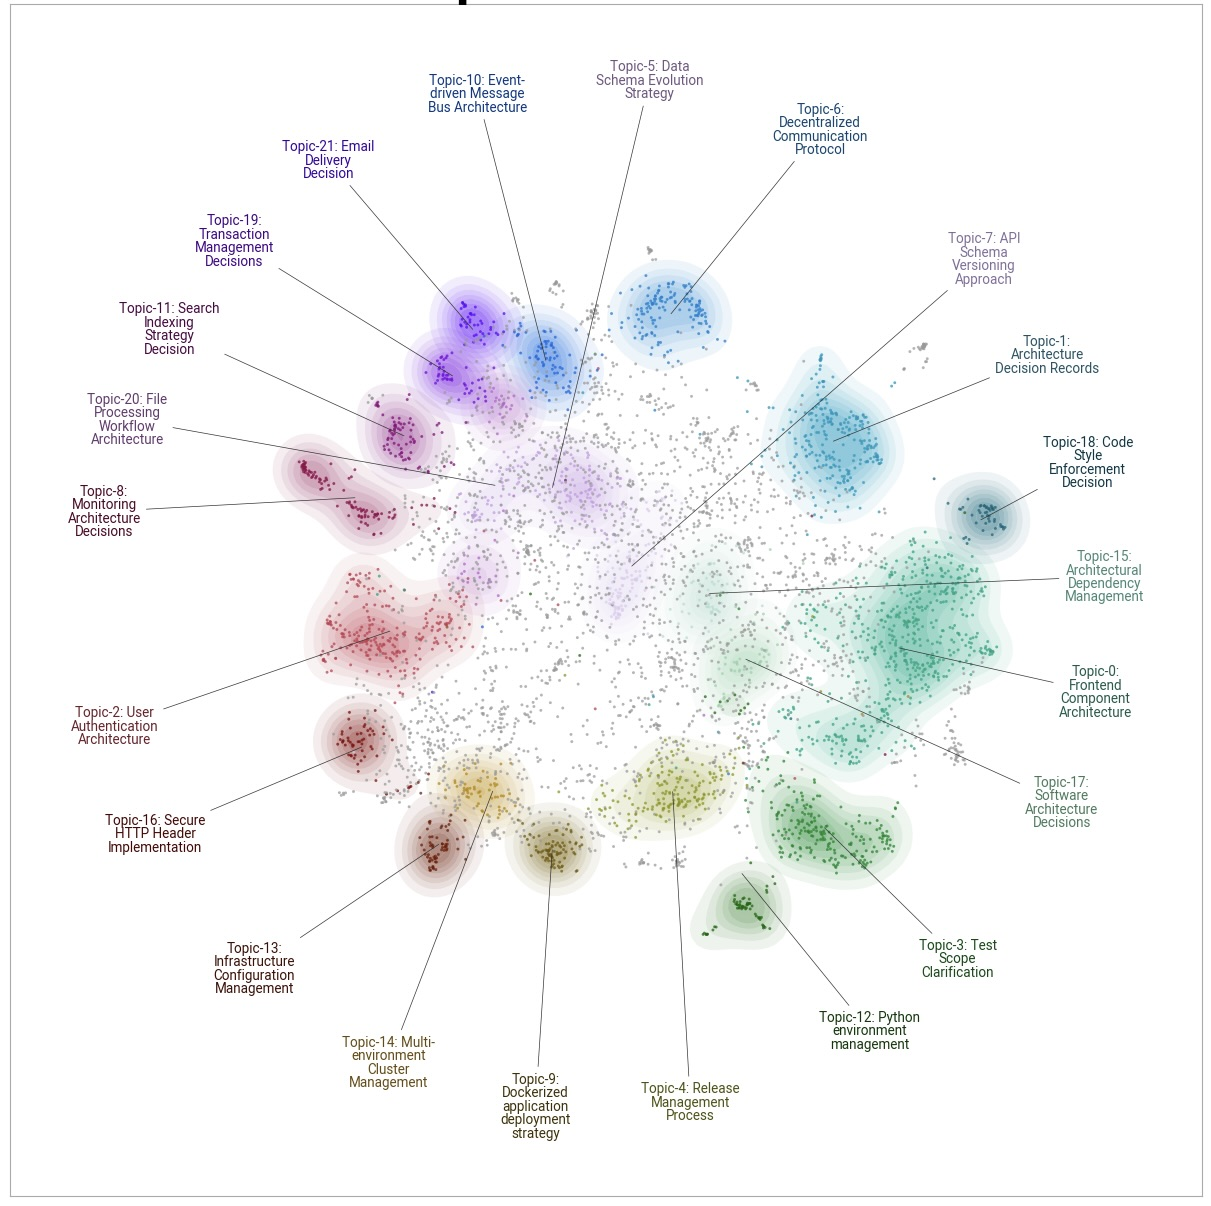
\includegraphics[scale=0.5]{figures/No Titles/datamap_original_no_title.jpeg}
            \caption{Datamap of documents from BerTopic analysis}
            \label{fig:bertopic_datamap_original}
        \end{figure}
        
        In the graph, documents' embeddings are projected in a two dimensional space with each data point representing one ADR. Clusters of documents are highlighted in different colors and their label is the result of the LLM representation model. 22 topics were identified based on the specified parameters. Around 15 of them are formed in tight clusters with clear semantic separation from the others. Those are mostly located around the edges of the graph. However, in the center of the graph, results are ambiguous and clusters are sparse. It is also important to note that 2575 ADRs, highlighted in grey in the center of the datamap, were not able to be assigned to a specific topic. Taking a closer look at the documents themselves by zooming in figure \ref{fig:docs_original}, the center also appears sparse with many documents that have not been classified. 
        
        \begin{figure}[h]
            \centering
            \hspace*{-2.2cm} 
            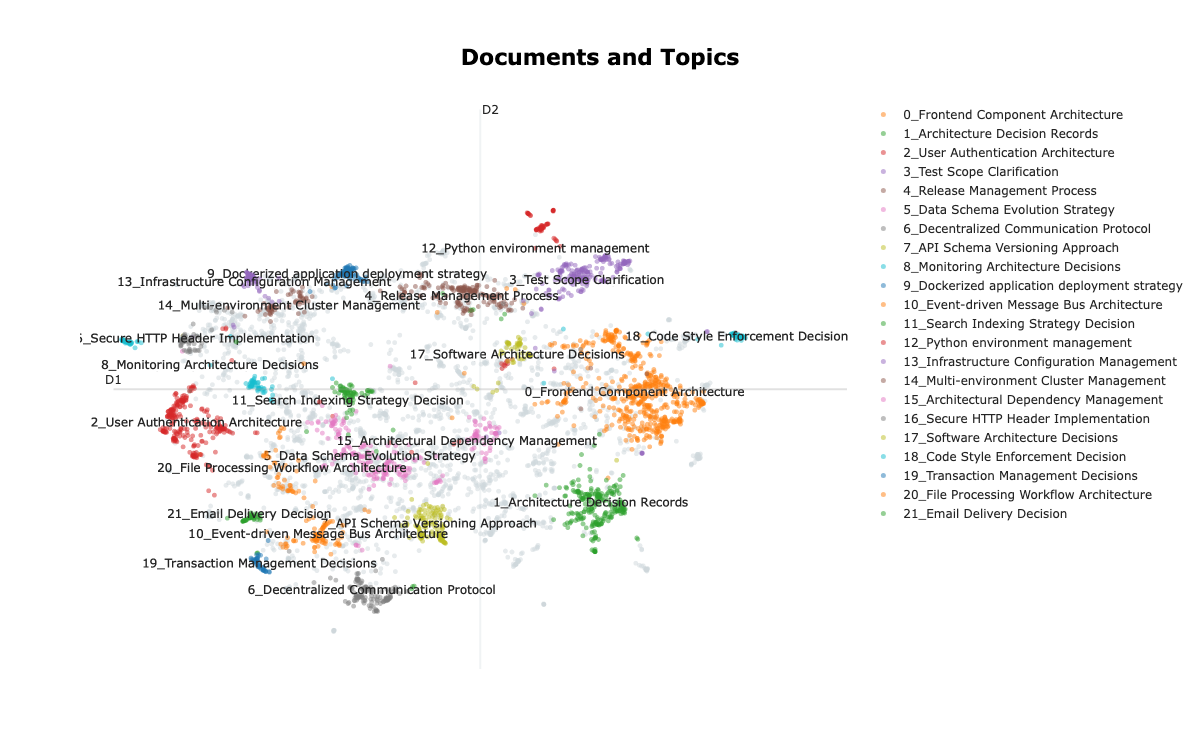
\includegraphics[scale=0.65]{figures/BerTopic_Original/docs_original.jpeg}
            \caption{Document embedding representation from BerTopic analysis}
            \label{fig:docs_original}
        \end{figure}
        
        However, the model seems to have captured semantic similarities in ADRs that serve a clear purpose, especially in certain areas like infrastructure management as presented in in figure \ref{fig:infra_docs}.

        \begin{figure}[h]
            \centering
            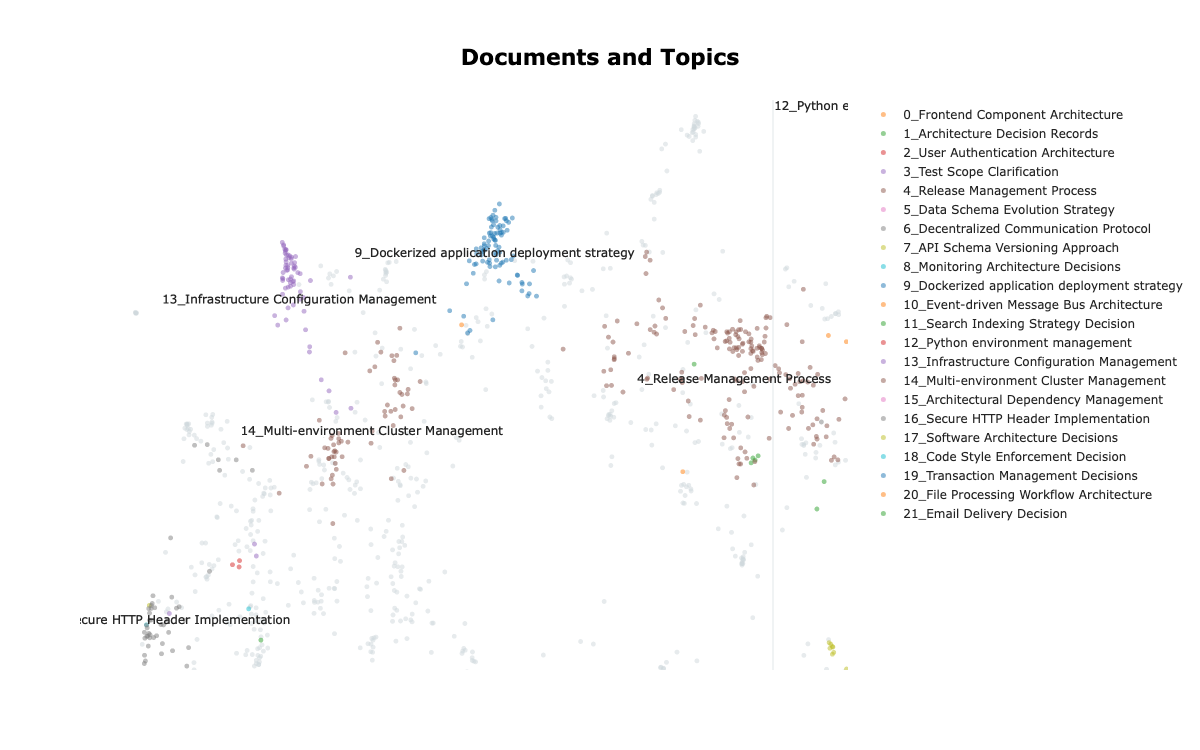
\includegraphics[scale=0.5]{figures/BerTopic_Original/zoomed_docs_infra.jpeg}
            \caption{ADRs related to cloud and infrastructure are located  closer in the embedding space}
            \label{fig:infra_docs}
        \end{figure}
        
        Examining the topics from a different perspective, a similarity matrix can be created to determine how clearly the topics have been separated by the model. This can also provide insights into the quality of the labels derived from the LLM, as conceptually similar topics should have a high similarity score and vise versa. The results are presented in figure \ref{fig:similarity_matrix_orginal}. 
        
        \begin{figure}[h]
            \centering
            \hspace*{-2cm} 
            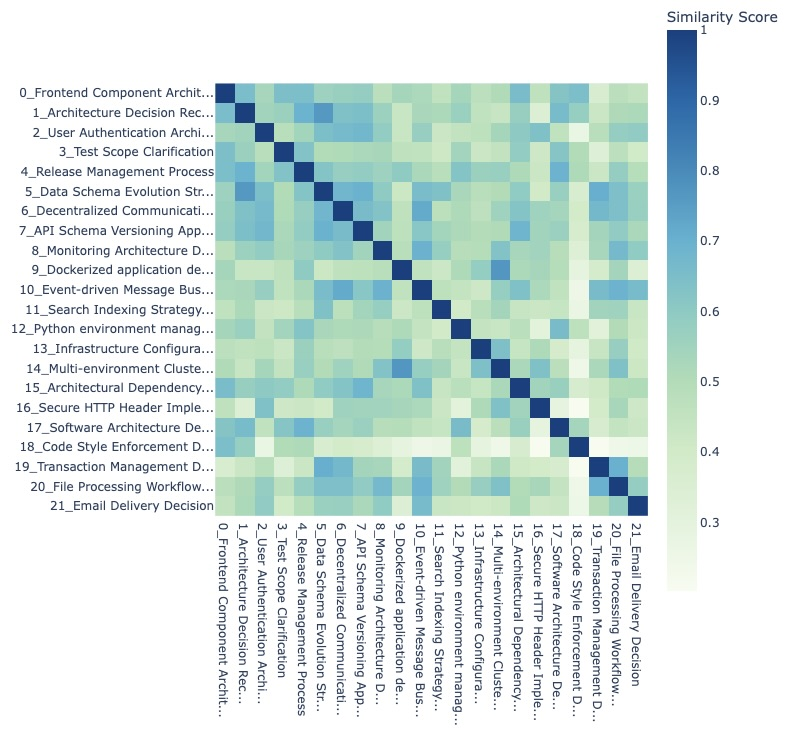
\includegraphics[scale=0.55]{figures/No Titles/heatmap_original_no_title.jpeg}
            \caption{ADR topic similarity matrix}
            \label{fig:similarity_matrix_orginal}
        \end{figure}
        
        Following the previous patterns, some topics appear to be clearly separated and others intertwined. For example, decisions about database transaction management and data schema evolution have a high similarity score of 0.7, whereas architectural decisions about containerization and code style formats present a lower score of 0.28. An observation can be made, from the color distribution and scale in the matrix, that many topic pairs, including irrelevant ones, have relatively high similarity, with the lowest being close to 0.2. The lowest score is related to code styling formats and the secure HTTP header implementation document cluster, while the highest, approaching 0.77 is compares dockerized application architectural decisions with decisions related to kubernetes cluster management. The high correlation, may be attributed to the similarity of the general theme of ADRs, with it being software architecture.

        To enhance the clarity of the results and create larger, more information-rich clusters, outlier reduction was applied to the topics, ensuring that only semantically similar documents were assigned to each cluster following the initial analysis. By utilizing the pre-calculated probabilities of an unlabeled document's likelihood of belonging to a specific cluster, the number of outliers was reduced to 704. The similarity threshold was set at 10\%, meaning outlier ADRs were included in the nearest topic cluster as long as they shared at least 10\% similarity. This low similarity threshold was chosen to maximize the number of documents assigned to a topic while isolating true outliers for further examination . The updated topic and document graph can be seen in figure \ref{fig:docs_reduced}.
        
        Topics now cover larger areas in the embedding space and there is more topic coverage in the center parts of the axes. Topic clusters have been extended to include ADRs with more distance, modifying their initial state. From a visual perspective, clusters do not appear overly altered although outliers have been reduced by 72\% which indicates promising results. The remaining outliers are also more apparent, indicated in grey data points and will be used for later analysis to determine the reason for their low similarity.

        \begin{figure}[h!]
            \centering
            \hspace*{-2.2cm} 
            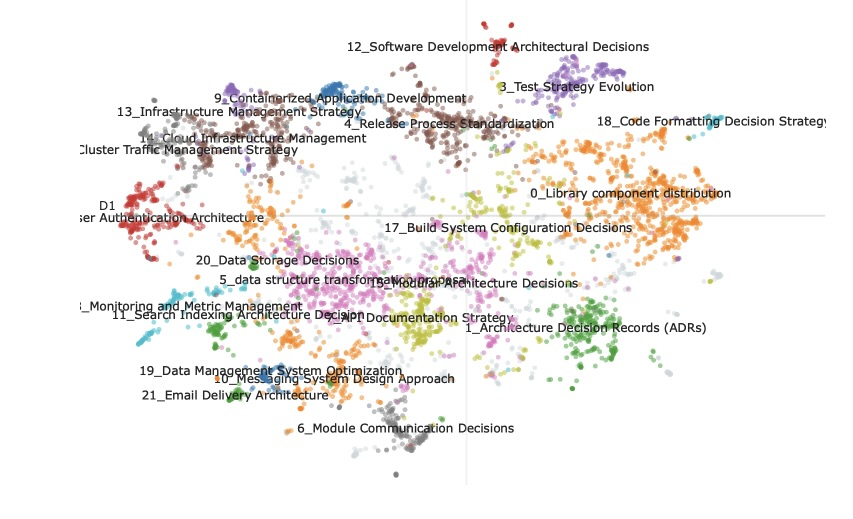
\includegraphics[scale=0.65]{figures/BerTopic_Reduced/docs_reduced_outliers.jpeg}
            \caption{Document embedding representation after outlier reduction}
            \label{fig:docs_reduced}
        \end{figure}

        In regards to topic similarity, the newly introduced documents, increased cluster diversity, indicated by the lowered similarity scores across all pairs of topics in figure \ref{fig:similarity_matrix_reduced}. This also slightly modified their respective representation labels. Semantically similar pairs also retained their higher score while irrelevant pair scores were reduced significantly, with the minimum being 0.02 between testing strategy decisions and library code component management,  indicating clearer topic separation. 

        \begin{figure}[h]
            \centering
            \hspace*{-2cm} 
            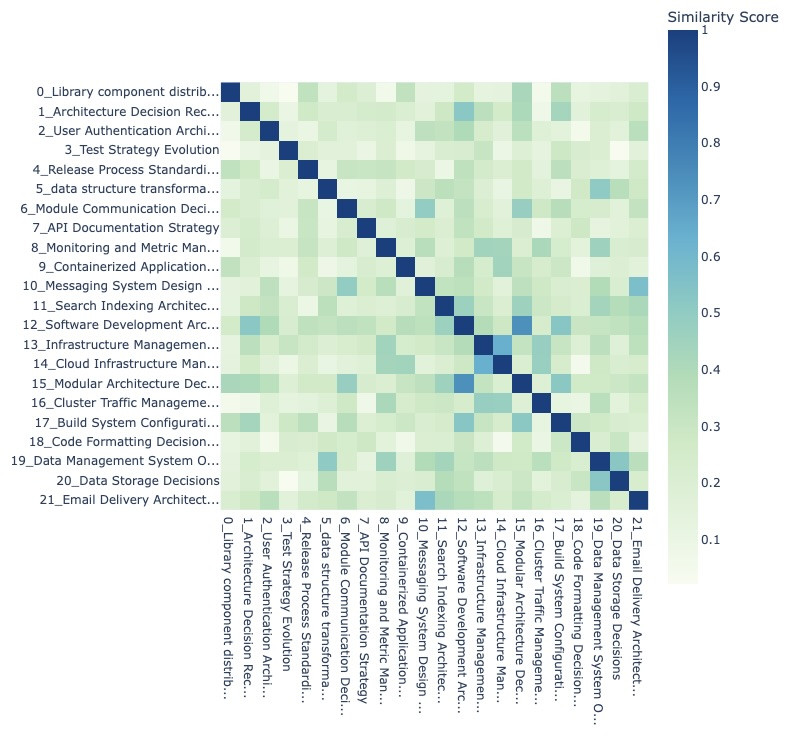
\includegraphics[scale=0.55]{figures/No Titles/similarity_matrix_reduced_outliers_no_title.jpeg}
            \caption{ADR reduced outlier topic similarity matrix}
            \label{fig:similarity_matrix_reduced}
        \end{figure}

        All research questions were answered using the results after the outlier reduction due to improved clarity. RQ3 also considered only the 704 final outliers as the filtering ensured their high degree of dissimilarity. A complete representation of the defined topics can be found in table 6.1.
        After closer examination of keywords and representative documents, five topics have been manually renamed from the original LLM representation. Topic ``Library component distribution'' has been renamed to ``Frontend Component and Design Decisions'' and ``Software Development Architectural Decisions'' has been changed to ``Python Development Decisions'' in line with its keyword representation. The latter, was modified drastically due to the LLM prompt explicitly forbidding the usage of names of specific technologies. Furthermore, ``Module Communication Decisions'' was renamed to ``Distributed Systems Communication Decisions'' due to the vast majority of documents referring to distributed system decisions such as blockchain node communication. Lastly, ``Infrastructure Management Strategy'' was renamed ``Infrastructure as Code Decisions'' and ``API Documentation Strategy Strategy was transformed to ``API Design Strategy'' to match their representative documents. 
        
        \begin{longtable}{|m{5cm}|c|c|c|c|c|c|}
    \hline
    % Nygard , Tyree \& Akerman , Alexandrian Pattern, Business Case, MADR , Planguage
    \textbf{Feature} & \textbf{NY} & \textbf{TA} & \textbf{AP} & \textbf{BC} & \textbf{MD} & \textbf{PL} \\
    \hline
    \textbf{Title} & + & + & - & + & + & + \\
    \hline
    \textbf{Status} & + & + & - & + & + & + \\
    \hline
    \textbf{Context/Background} & + & - & + & + & + & + \\
    \hline
    \textbf{Problem/Issue} & + & + & + & + & + & + \\
    \hline
    \textbf{Forces/Decision Drivers} & - & - & + & - & + & - \\
    \hline
    \textbf{Decision} & + & + & + & + & + & + \\
    \hline
    \textbf{Options} & - & - & - & + & + & + \\
    \hline
    \textbf{Solution} & + & + & + & + & + & + \\
    \hline
    \textbf{Consequences
    /Implications} & + & + & + & + & + & + \\
    \hline
    \textbf{Motivation/
    Rationale} & - & + & - & - & + & + \\
    \hline
    \textbf{Assumptions} & - & + & - & - & - & - \\
    \hline
    \textbf{Related Decisions} & - & + & - & - & - & - \\
    \hline
    \textbf{Stakeholders} & - & - & - & - & - & + \\
    \hline
    \textbf{Pros and Cons} & - & - & - & - & + & - \\
    \hline
    \caption{Comparison of ADR Templates}
    \label{table:adr_template_comparison}
\end{longtable}

    \section{RQ1: What are the most frequently discussed software architecture topics in ADRs?}

        To determine which topics are more prevalent in our dataset, the total number of ADRs per topic were counted and sorted. Then, for each topic, its document count was expressed as a percentage of total ADRs in the data. The results are presented in the bar chart in figure \ref{fig:docs_per_topic_percentage}. We will take a look at some notable ones. At a first glance, topics seem to be evenly distributed. The most frequent topic by a large margin, totaling 14.34\% of all documents is represented by the title ``Frontend Component and Design Decisions'', its most frequent keywords are ``react'', ``component'', ``typescript'', ``npm'', ``framework'', ``frontend'', ``dependency'', ``design'', ``development'', ``angular''. This is the large orange cluster in figure \ref{fig:docs_reduced} that contains 770 ADRs. The second most frequent topic is labeled ``Database Schema Management and Data Migration'' and its keywords are ``database'', ``schema'', ``sql'', ``metadata'', ``implementation'', ``data'', ``information'', ``structure'', ``migration'', ``json'' and seems to describe data related decisions such as storage and database structure. Other interesting topics include the topic labeled ``User Authentication Architecture'' that brings up security related topics at a 4,61\%, described by keywords as ``access control'', ``authorization'',``oauth'', ``authentication'',``openid'', ``access token'',``security'' and the topic named ``Cloud Infrastructure Management'' with ``kubernetes'', at a 5.4\% with ``cloud platform'', ``cluster'',``elasticsearch'', ``docker'',``pod'',``aws'', as dominant words. An ADR topic about architectural decisions and ADR themselves seems to emerge as the 5th most frequent topic containing 5.14\% of total documents. From its keywords, ``architectural record'', ``documentation'', ``changelog'', ``record architecture'', ``document'', ``structure'' it seems to also revolve around documentation and probably represents some of the first ADRs in each repository that state the need for ADRs and their usage moving forward. From the file cleaning process, at least 35 of those ADRs were identified. Lastly, the least frequent topics are related to email monitoring and notifications and code formatting conventions as indicated by their titles ``Code Formatting Decision Strategy'' and ``Email Delivery Architecture'' at percentages of 0.80 and 0.93 respectively. 

        \begin{figure}[h!]
            \centering
            \hspace*{-2,8cm} 
            \includegraphics[scale=0.50]{figures/topic_percentages_final2.png}
            \caption{Documents per topic as a percentage of total documents}
            \label{fig:docs_per_topic_percentage}
        \end{figure}

        A sorting of the identified topics, as they relate to software engineering domains and practices can be seen in figure \ref{fig:topic_tree_sort_RQ1} . The categorization is based on the  on version 3 of the Software Engineering Body of Knowledge Guide (SWEBOK) \cite{swebok_v3}.

        \begin{sidewaysfigure}[p]
            \hspace*{-0.8cm} 
            \centering
            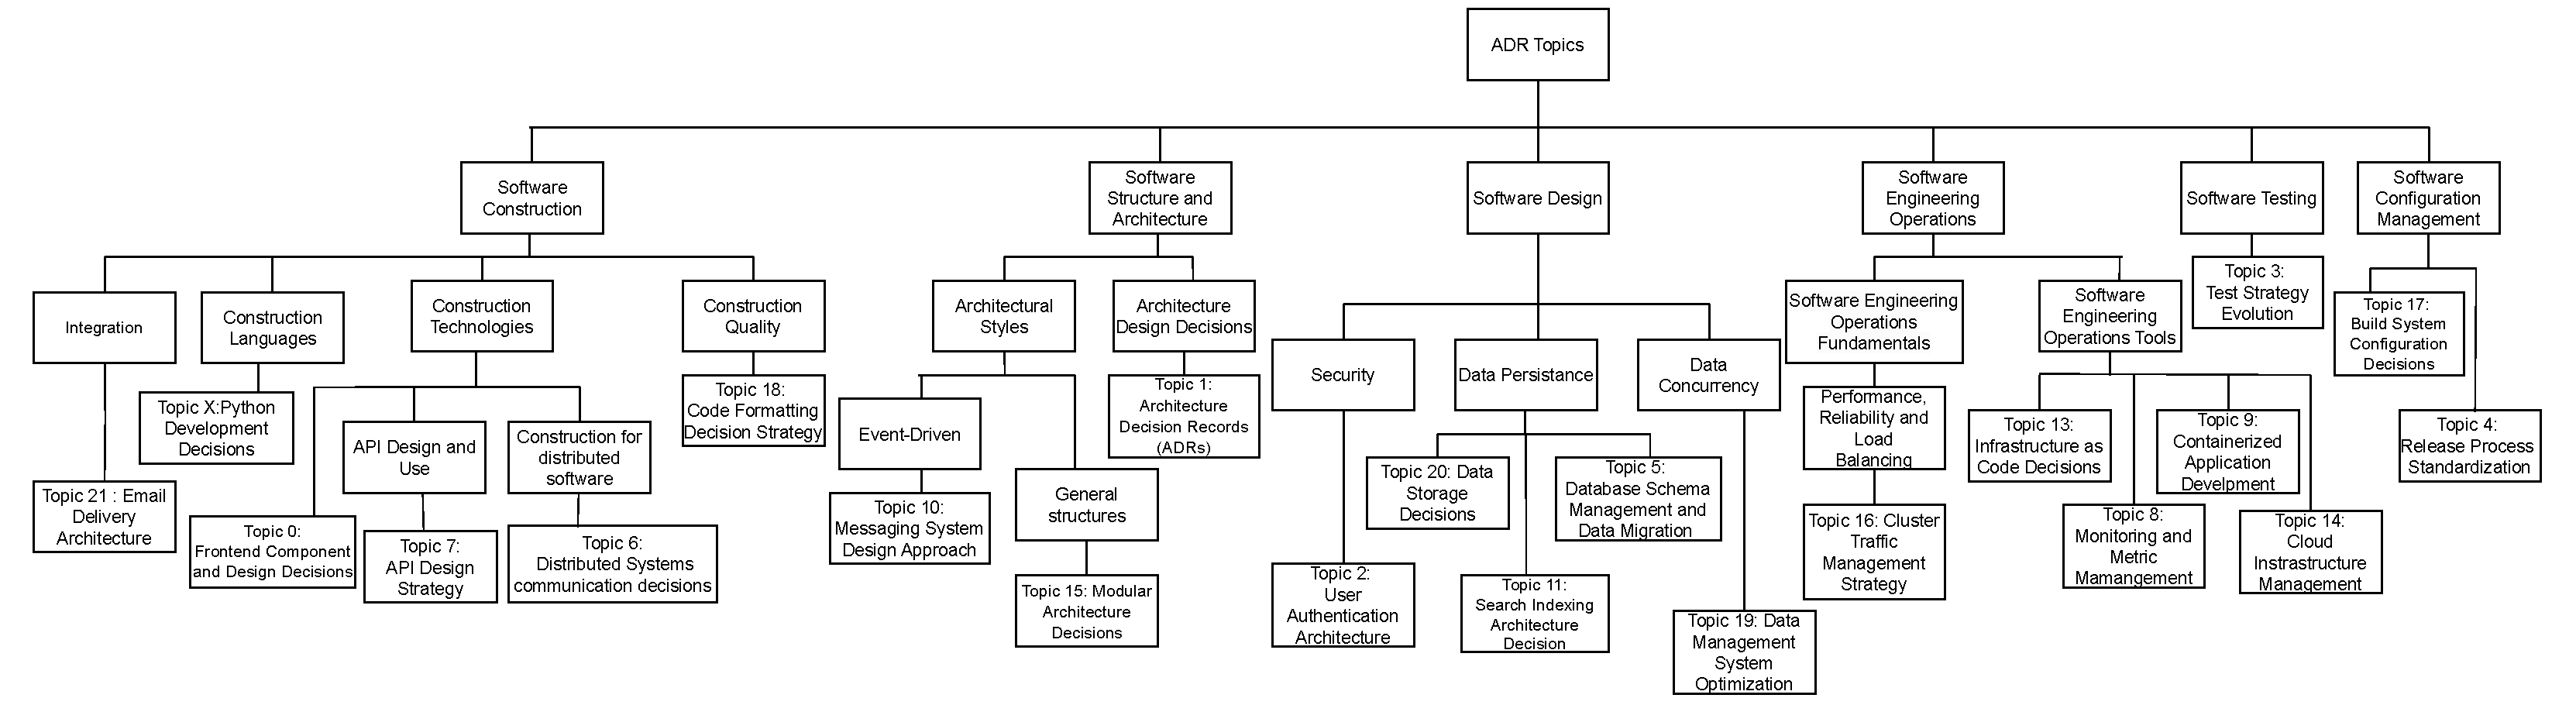
\includegraphics[scale=0.50]{figures/RQ1_sort_final.drawio.pdf}
            \caption{ADR topic sorting}
            \label{fig:topic_tree_sort_RQ1}
            \hspace*{-2cm} 
        \end{sidewaysfigure}

    \section{RQ2: How many topics from the general software architecture space are present in the ADRs?}

        Before determining which subset of topics from ADRs exist in the software architecture landscape, we must define a set of broad categories that architects have to consider when making design decisions. This is not a trivial task, as many trends, styles and general topics are implicit and documentation about actual architectural practices and decisions is limited.\cite{arch_patterns_in_practice_TOPICS}. In addition, design decisions can also be made to satisfy system attributes. Prominent attributes include availability, usability, performance, security, testability, modifiability and usability which are not topics but more so, systemic qualities that satisfy implied system or business needs \cite{patters+quality_requirements+tactics}.
        
        Architectural patterns, on the other hand, refer to a set of pre-defined styles and techniques for solving common reoccurring architectural problems, are more tangible but system-specific \cite{Patterns+ArchDecisions}. Some popular patterns are Layers, Pipes-Filters, Model View Controller (MVC), Broker and Client–Server and are derived from the component-connector conceptual model \cite{survey_arch_patterns}. These aspects of decisions alone, do not constitute valid categorizations for our analysis as they refer to concepts that are either too implementation-specific or too broad. 
        
        Combining the two, we get architectural tactics. Architectural tactics ``serve as the
        meeting point between the quality attributes and the software architecture`` \cite{patters+quality_requirements+tactics}. Tactics are essentially specific measures taken to improve the quality attributes of the system. For example, an architect may decide to incorporate authentication and authorization into a system which in turn enhances security. Or referring to the findings of the previous question, a project may decide to use a specific frontend development framework in order to promote reusability if the framework allows for reusable code components. A comprehensive collection of tactics to satisfy specific system quality attributes, can be found in the Software Architecture in Practice book \cite{software_arch_in_practice_book}. 
        
        To answer RQ2, each topic identified from the previous question's results was examined and interpreted based on its frequent keywords and LLM representation, aiming to match it with any specific architectural pattern, tactic, or technique that fulfills a particular quality attribute. If the associated quality attributes are not immediately clear, a deeper dive into the topic was necessary, reviewing its representative ADRs, and attempting to identify several potential quality attributes, as we can't conclusively determine the true intents of each ADR author. This is an empirical approximation since many ADRs mentioned the potential adoption of very specific technologies and tools rather than architectural patterns and architectures of system components, which is not ideal when trying to examine architectural styles used. Furthermore, many topics refer to sub-processes and conceptually lower level techniques and some patterns were identifiable in subsets of the topic's documents.
        
        Future research could try to increase the total number of topics and closely examine each cluster to uncover additional patterns that may be overshadowed by more prominent ones within the cluster. This approach was not used as more clusters produced less comprehensive topics of ADRs and the sample size of each topic decreased by several orders of magnitude. The results of the comparison are presented in table \ref{table:topic_tactic}. Two semantically similar topics have been merged into larger categories, namely ``data management'' and ``cloud infrastructure'', reducing the total number of considered topics to 20.

        % { \small
%         \begin{longtable}{|p{3.8cm}|p{3cm}|p{2.2cm}|p{2.57cm}|p{2.8cm}|}
%         \caption{Topic Tactic Analysis}
%         \label{table:topic_tactic}
%         \hline
%         \textbf{Topic} & \textbf{Tactic} & \textbf{Pattern} & \textbf{Style} & \textbf{Quality Attribute} \\
%         \hline
%         \endfirsthead
    
%         \hline
%         \textbf{Topic} & \textbf{Tactic} & \textbf{Pattern} & \textbf{Style} & \textbf{Quality Attribute} \\
%         \hline
%         \endhead
        
%         \hline
%         \endfoot
        
%         \hline
%         \endlastfoot
        
%         Frontend Component and Design Decisions & Modularization & Component-Based & N/A & Reusability, Modifiability \\
%         \hline
%         Architecture Decision Records (ADRs) & Documentation & N/A & N/A & Maintainability \\
%         \hline
%         User Authentication Architecture & Authentication and Authorization & N/A & N/A & Security \\
%         \hline
%         Test Strategy Evolution & Automated Testing & N/A & N/A & Testability, Modifiability \\
%         \hline
%         Release Process Standardization & Continuous Integration/Continuous Deployment (CI/CD) & N/A & N/A & Maintainability, Reliability \\
%         \hline
%         Database Schema Management and Data Management System Optimization & Database Normalization, Data Optimization & N/A & Data-Centric & Maintainability, Performance, Efficiency \\
%         \hline
%         Module Communication Decisions & Asynchronous Messaging & Publish-Subscribe & Event-Driven & Performance, Scalability \\
%         \hline
%         API Documentation and Design Strategy & API Documentation & RESTful API & Representational State Transfer (REST) & Interoperability, Usability \\
%         \hline
%         Monitoring and Metric Management & Monitoring and Logging & N/A & N/A & Reliability, Maintainability \\
%         \hline
%         Containerized and Cloud Infrastructure Management & Containerization, Container Orchestration & Microservices & Service-Oriented Architecture (SOA) & Scalability, Availability, Modifiability \\
%         \hline
%         Messaging System Design Approach & Event-Driven Messaging & Event-Driven & N/A & Performance, Scalability \\
%         \hline
%         Search Indexing Architecture Decision & Indexing & N/A & N/A & Performance, Efficiency \\
%         \hline
%         Python Development Decisions & Scripting & N/A & N/A & Maintainability, Flexibility \\
%         \hline
%         Infrastructure Management Strategy & Infrastructure as Code & N/A & N/A & Scalability, Efficiency \\
%         \hline
%         Modular Architecture Decisions & Modularization & Modular Architecture & N/A & Modifiability, Reusability \\
%         \hline
%         Cluster Traffic and Load Management & Load Balancing & N/A & N/A & Performance, Availability \\
%         \hline
%         Build System Configuration Decisions & Configuration Management & N/A & N/A & Maintainability, Reliability \\
%         \hline
%         Code Formatting Decision Strategy & Code Quality & N/A & N/A & Maintainability, Readability \\
%         \hline
%         Data Storage Decisions & Data Storage Management & N/A & N/A & Performance, Data Integrity \\
%         \hline
%         Email Delivery Architecture & Notification Management & N/A & N/A & Usability, Reliability \\
%         \hline
%         \end{longtable}
%     }



{\small
    \begin{longtable}{|p{5cm}|p{6cm}|p{3cm}|}
        \caption{Topic Tactic Analysis}
        \label{table:topic_tactic}
        \hline
        \textbf{Topic} & \textbf{Tactic/Pattern/Style} & \textbf{Quality Attribute} \\
        \hline
        \endfirsthead
        
        \hline
        \textbf{Topic} & \textbf{Tactic/Pattern/Style} & \textbf{Quality Attribute} \\
        \hline
        \endhead
        
        \hline
        \endfoot
        
        \hline
        \endlastfoot
        
        Frontend Component and Design Decisions & Modularization, Component-Based, Model-View-Controller (MVC) & Reusability, Modifiability) \\
        \hline
        Architecture Decision Records (ADRs) & Documentation & Maintainability \\
        \hline
        User Authentication Architecture & Authentication and Authorization & Security \\
        \hline
        Test Strategy Evolution & Automated Testing & Testability, Modifiability \\
        \hline
        Release Process Standardization & Continuous Integration/Continuous Deployment (CI/CD) & Maintainability, Reliability \\
        \hline
        Database Schema Management and Data Management System Optimization & Pipes and Filters, Big Data Architecture, Database Normalization & Maintainability, Performance, Efficiency \\
        \hline
        Distributed Systems Communication Decisions & Peer-to-Peer, Distributed Architecture & Security, Reliability \\
        \hline
        API Documentation and Design Strategy & API Documentation, Client-Server, Representational State Transfer (REST) & Interoperability, Usability \\
        \hline
        Monitoring and Metric Management & Monitoring and Logging & Reliability, Maintainability \\
        \hline
        Containerized and Cloud Infrastructure Management & Containerization, Container Orchestration, Microservices, Service-Oriented Architecture (SOA), Cloud Computing Architecture & Scalability, Availability, Modifiability \\
        \hline
        Messaging System Design Approach & Event-Driven, Broker Model & Performance, Scalability \\
        \hline
        Search Indexing Architecture Decision & Indexing & Performance, Efficiency \\
        \hline
        Python Development Decisions & Scripting & Maintainability, Flexibility \\
        \hline
        Infrastructure Management Strategy & Infrastructure as Code & Scalability, Efficiency \\
        \hline
        Modular Architecture Decisions & Model-View-Controller (MVC), Modularization, Modular Architecture & Modifiability, Reusability \\
        \hline
        Cluster Traffic and Load Management & Load Balancing, Cloud Computing Architecture & Performance, Availability \\
        \hline
        Build System Configuration Decisions & Configuration Management & Maintainability, Reliability \\
        \hline
        Code Formatting Decision Strategy & Code Quality & Maintainability, Readability \\
        \hline
        Email Delivery Architecture & Client-Server, Notification Management & Usability, Reliability \\
        \hline
    \end{longtable}
}

        Overall, many of the most popular tactics, styles and patterns are present in the data indicating that open source projects mostly adhere to the same architecture principles. The diversity of architectural topics is also notable. Factoring in the percentage share of each topic relative to the tactic used, the Model-View-Controller (MVC) model is widely used, with many ADRs also referencing cloud computing topics and patterns. This confirms the findings from a recent study on trends in software architecture.\footnote{https://www.oreilly.com/radar/the-topics-to-watch-in-software-architecture/} Additionally, other well-established patterns such as Microservices, RESTful API, and Service-Oriented Architecture (SOA) are represented. The same study, conducted at the O’Reilly Software Architecture Conference in 2019, a year before our dataset was extracted, highlighted significant topics including microservices, testing, data, and monitoring, which matches our findings. On the opposite side, many ADRs, heavily focused on web development decisions which saw a heavy decline in topic trend. Notable missing topics include AI and machine learning, as well as a broader coverage of security practices and patterns such as the Layered Pattern, Blackboard, and Monolithic applications.
        
    \section{RQ3: Which ADR topics cannot be classified, and what are the reasons behind this?}
        From the main analysis, 707 ADRs could not be classified to a specific topic so they remained outliers. This could have been a result of several factors. Firstly, the minimum cluster size was initially set to 40 documents, meaning that topics present in less than 40 ADRs were considered outliers due to their limited presence in the dataset. Furthermore, outlier ADRs could refer to very specific project or technology decisions, which could disrupt the representations of larger clusters, making them more challenging to analyze semantically. As a result, these ADRs were excluded.
        
        For the outlier analysis, ADRs that were not assigned to topics were isolated and further topic modelling was performed on them to uncover their themes. This time, the numbers of documents per cluster was lowered to 10 aiming to uncover niche, underrepresented topics in the main dataset. Since the LLM could not produce satisfactory representations, topics were identified based on their frequent keywords in the respective ADRs. The results are presented in figure \ref{fig:outlier_datamap}.
        
        ADRs were clustered into 17 evenly distributed topics comprising of 20-80 documents. Most clusters are clearly separated in the embedding space. Outliers seem to focus on more implementation-specific topics such as API designs as indicated by topic 9, referring to GraphQL, tools such as hosting platforms seen in topic 12 referring to Heroku, and other decisions about project tactics and techniques such as caching (topic 8), tenancy (topic 4) and payment handling (topic 2). Environment variable management, time handling and routing (topics 14, 5 and 13) are also notable topics that concerned architects but to a lesser degree. In summary, the ADRs remained unclassified due to their small number in the main dataset rather than their abstract nature. They represent valid topics and strategies in software engineering, indicating that they could be integrated into the main topics if the dataset were expanded with more documents.
        
        \begin{figure}[H]
            \centering
            \hspace*{-1.2cm} 
            \includegraphics[scale=0.55]{figures/outlier_datamap.png}
            \caption{Outlier Document Datamap}
            \label{fig:outlier_datamap}
        \end{figure}

    \newpage
    \section{Threats to Validity}
    This study, like any empirical research, faces several threats to validity that must be addressed. Firstly, the topic modelling approach relies heavily on its hyperparameters that can alter the results with each run. The hyperparameters chosen were deemed satisfactory after many trials and the assessment of quality of each run was subjective in nature \cite{subjective_topic_modelling}.

    In addition, preprocessing steps, although close to popular industry practices, relied on personal observation and choice when it comes to areas of word filtering. If excluded words were to be changed, the results may differ.
    
    Furthermore, the dataset consisted primarily of ADRs from open-source GitHub projects, which may not fully represent ADRs from proprietary or enterprise environments. Readers should exercise caution when extending these results to a broader context, especially considering the relatively small amounts of documents in the dataset.
    
    When it comes to topic representation, the use of LLMs for topic titles might not have captured the full semantic meaning of each ADR in each cluster, as only 4 of the ADRs were delivered as prompts to the model each time a label was generated, along with the most frequent keywords. The prompt used to make the requests to the model was also a result of fine tuning and in the end, highly subjective. This could potentially lead to oversimplification or misclassification and exact topic titles could not be replicated due to the LLMs non-deterministic nature.
    
    Lastly, it needs to be considered that the ADRs analyzed in this study, derived from a snapshot of the state of GitHub, that is evolving on a daily basis. The repositories used can be modified or deleted at any time, just like we observed in the dataset scrapping process, hindering the reproducability of the results.